\documentclass{report}
\usepackage[spanish]{babel}
\usepackage[margin=2cm]{geometry}
\usepackage{graphicx} % Required for inserting images
\usepackage{titlesec}
\usepackage{caption}

\titleformat{\section}
{\huge\bfseries}{\thesection.}{1em}{}
\titleformat{\subsection}
{\large\bfseries}{\thesubsection}{1em}{}


\title{\Huge{\textbf{Practica 1. Algoritmo genético para espacios continuos}}\\
\Large{\textbf{Algoritmos Bioinspirados}}}
\author{Diego Castillo Reyes\\Marthon Leobardo Yañez Martinez\\Aldo Escamilla Resendiz}

\graphicspath{{Imagenes/}}

\begin{document}
    \maketitle
    \newpage
    \section*{Introducción}
    En esta practica hemos implementado un algoritmo genético para resolver un problema de optimización en un espacio continuo. 
    El problema consiste en encontrar el mínimo de las funciones de Rosenbrock y Ackley, representadas por las siguientes ecuaciones respectivamente:
    \begin{equation}
        f(x)_{Rosenbrock} = \sum_{i=1}^{n-1} [100(x_{i+1} - x_{i}^2)^2 + (1 - x_{i})^2]
    \end{equation}
    \begin{equation}
        f(x)_{Ackley} = -20exp(-0.2\sqrt{\frac{1}{n}\sum_{i=1}^{n}x_{i}^2}) - exp(\frac{1}{n}\sum_{i=1}^{n}cos(2\pi x_{i})) + 20 + e
    \end{equation}

    Para llevar a cabo esta tarea, se optó por el lenguaje de programación Python debido a su versatilidad, facilidad de uso y a la gran cantidad de librerías que ofrece 
    para el manejo de arreglos y operaciones matemáticas. Además, se utilizó la librería \textit{matplotlib} para graficar las funciones y el comportamiento 
    del algoritmo genético.

    \section*{Desarrollo}
    El algoritmo se dividió en 6 funciones principales:
    \subsection*{Función de inicialización de población}
    \begin{figure}[h]
        \centering
        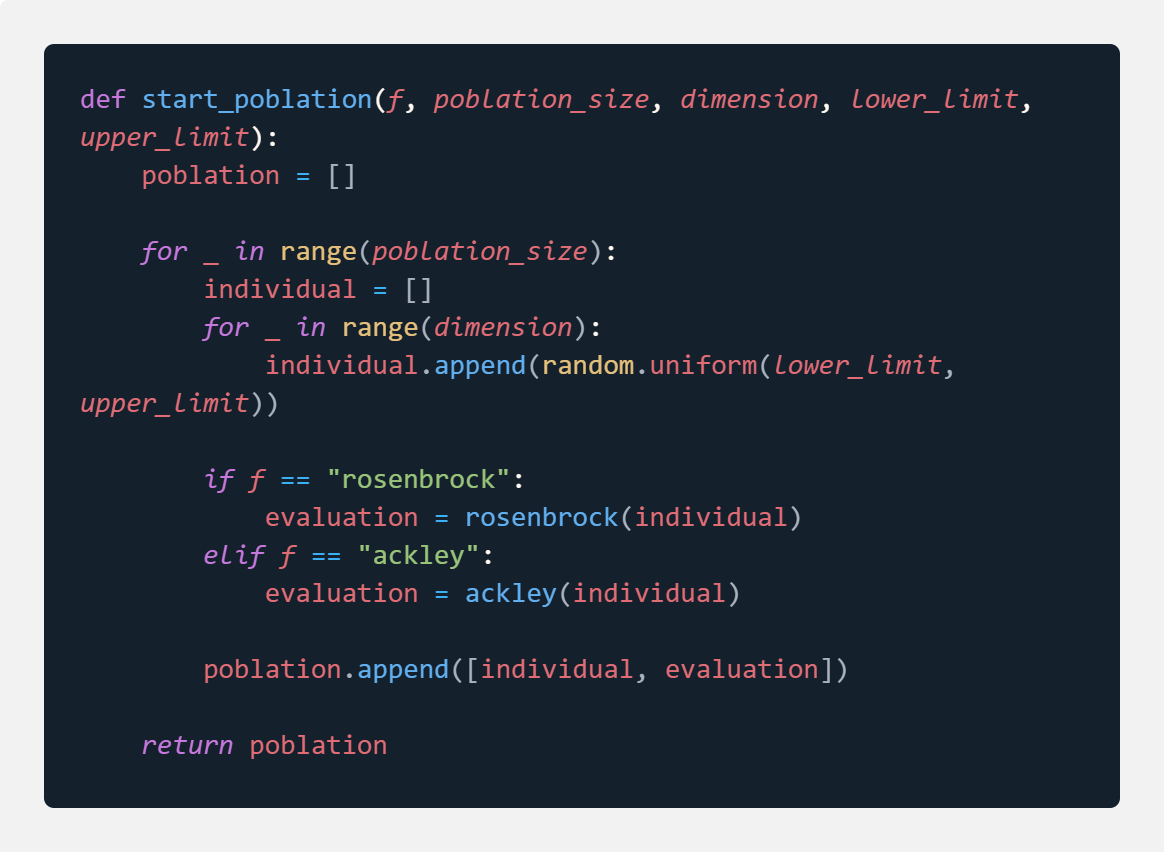
\includegraphics[width=0.5\textwidth]{funcionPoblacion.png}
        \caption{Función población}
    \end{figure}
    Esta función se utiliza para inicializar una población de individuos 
    con valores aleatorios en un rango específico dado por la función. La función toma cinco parámetros: el número de individuos, el número de variables,
    f, tamaño de la población, dimensión, limite inferior y limite superior.
    
    \begin{itemize}
        \item f: Es una cadena que especifica la función de aptitud que se utilizará, ya sea Rosenbrock o Ackley.
        \item tamaño de la población: Es el número de individuos que se generarán.
        \item dimensión: Es el número de variables que tendrá cada individuo.
        \item limite inferior: Es el valor mínimo que pueden tomar las variables de cada individuo.
        \item limite superior: Es el valor máximo que pueden tomar las variables de cada individuo.
    \end{itemize}
    
    La función comienza inicializando una población de lista vacía para contener la población de individuos. Luego ingresa a un bucle que ejecuta las veces de individuos seleccionados. En cada iteración de este ciclo, se crea un nuevo individuo.

    Un individuo se representa como una lista de números de dimensión. Cada número es un flotante aleatorio generado por la función random.uniform, que devuelve un flotante aleatorio dentro del rango especificado por el límite inferior y límite superior.
    Una vez que se crea un individuo, su aptitud se evalúa utilizando la función de aptitud especificada. Si f es Rosenbrock, la función Rosenbrock se llama con el individuo como argumento. Si f es Ackley, en su lugar se llama a la función Ackley. La evaluación de aptitud se almacena en la evaluación de variables.

    Finalmente, el individuo y su evaluación de aptitud se agregan como un par a la lista de población. Este proceso se repite hasta que se hayan creado y evaluado los individuos del tamaño de la población.
    La función devuelve la lista de población, que ahora contiene pares del tamaño de la población, cada uno de los cuales consta de un individuo y su evaluación de aptitud.

    \subsection*{Función que define las parejas}
    \begin{figure}[h]
        \centering
        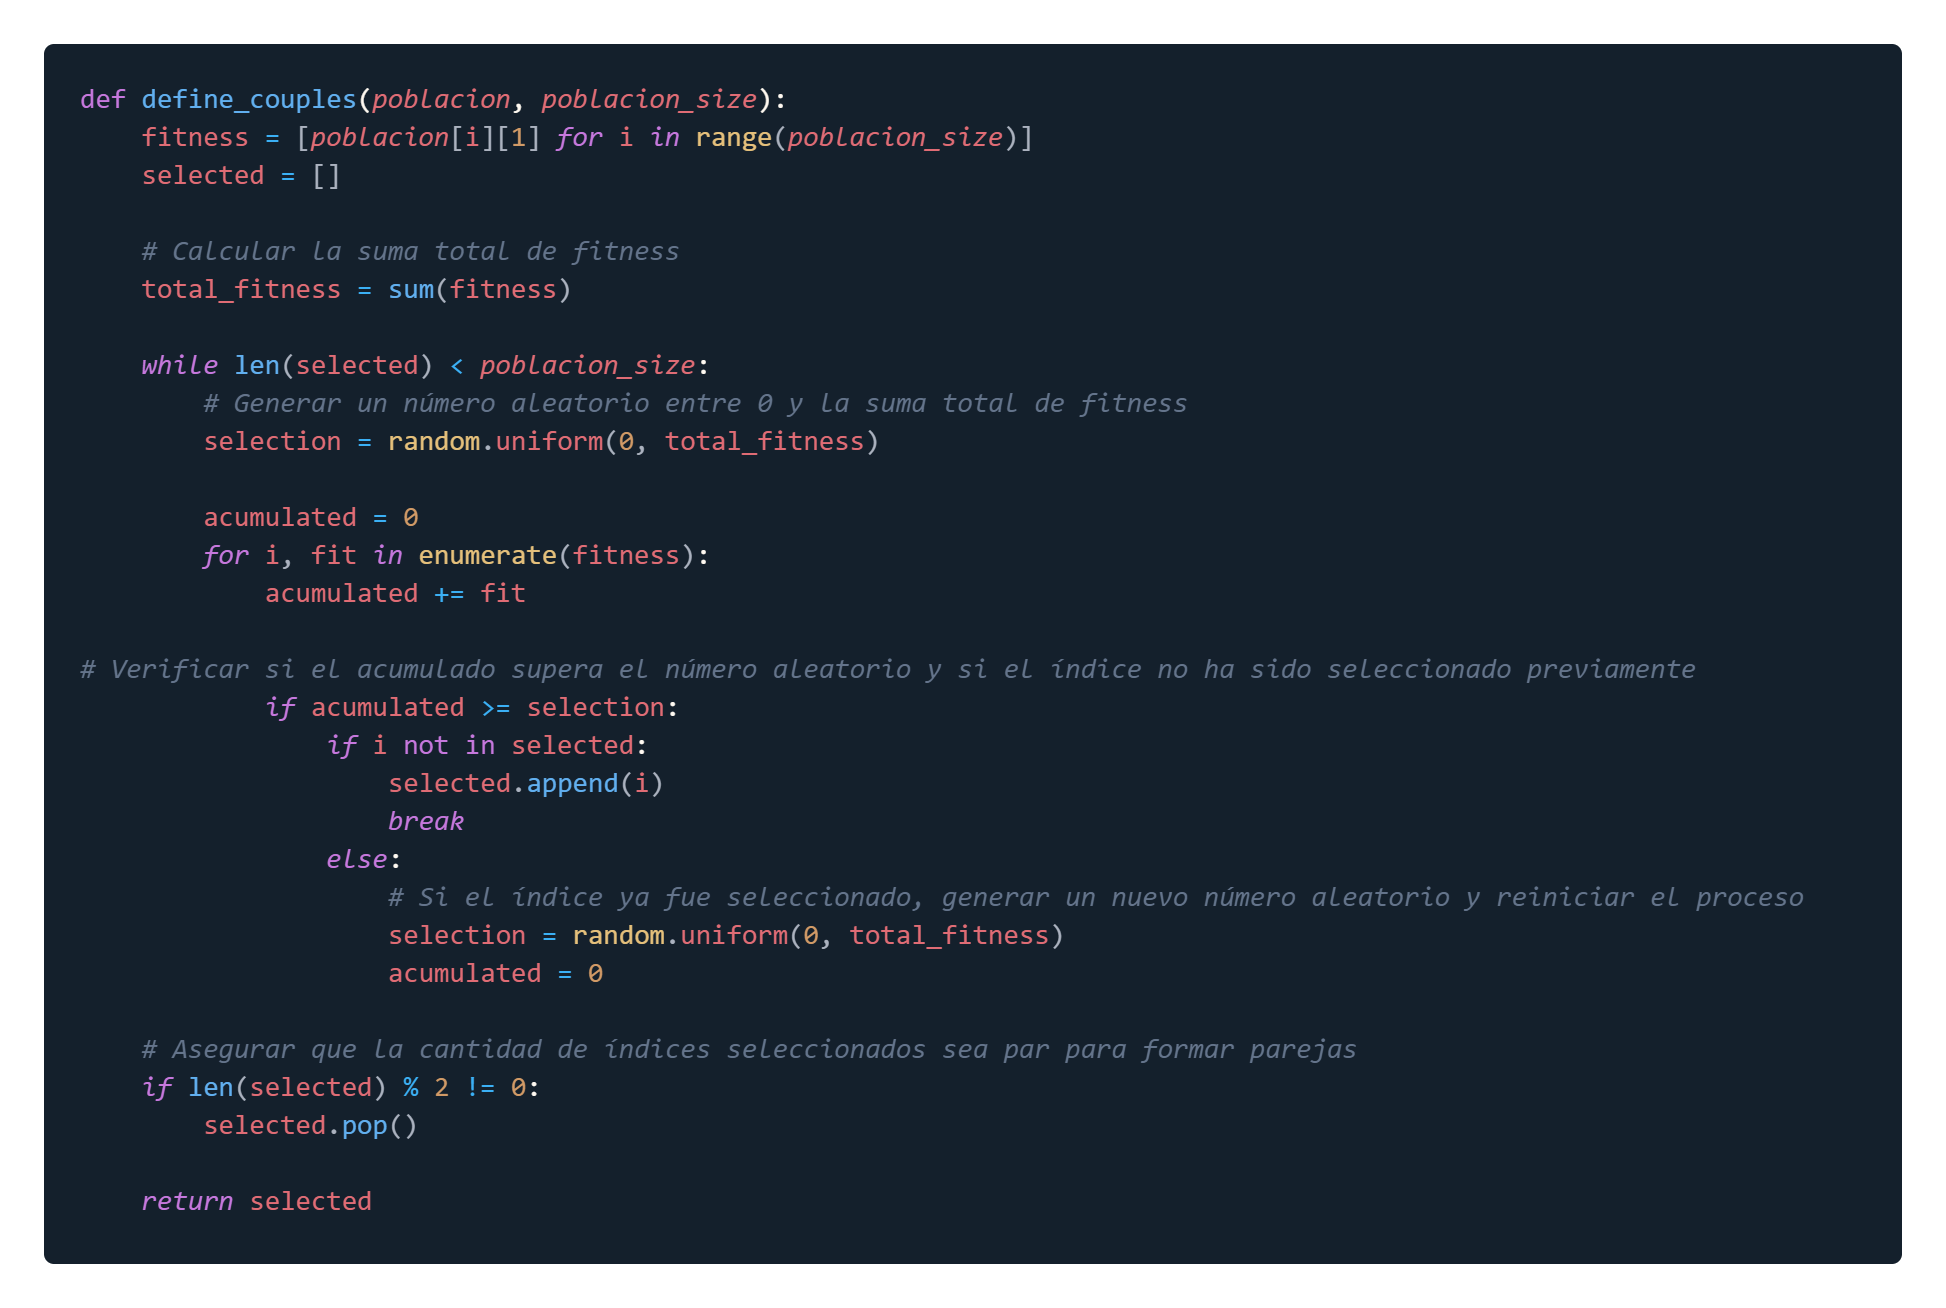
\includegraphics[width=0.5\textwidth]{funcionParejas.png}
        \caption{Función parejas}
    \end{figure}
    La función recibe como parámetros la población y el número de parejas que se seleccionarán. 
    %crea una lista no ordenada detallando los parámetros

    \begin{itemize}
        \item población: Es la lista de individuos que se cruzarán.
        \item número de parejas: Es el número de parejas que se seleccionarán.
    \end{itemize}
    
    Esta función se utiliza para seleccionar las parejas de individuos que se cruzarán para generar una nueva población. La función toma dos parámetros: la población y el número de parejas que se seleccionarán.
    La función empieza creando la lista fitness, que contiene los valores de ajuste de la población. Posteriormente crea la lista de seleccionados donde se almacenarán los indices de los individuos seleccionados.
    Luego, se ingresa a un bucle que se ejecuta el número de veces que se seleccionarán parejas. En cada iteración de este ciclo, se selecciona una pareja de individuos y se agrega a la lista de acumulados.
    Después de seleccionar una pareja, comprueba que la lista de las parejas que se cruzarán sea un número par y si no lo es, se elimina al ultimo individuo de la lista de seleccionados.
    Finalmente, la función devuelve la lista de seleccionados, que contiene los índices de los individuos seleccionados para cruzarse.
    
    \newpage
    \subsection*{Función de cruza}
    \begin{figure}[h]
        \centering
        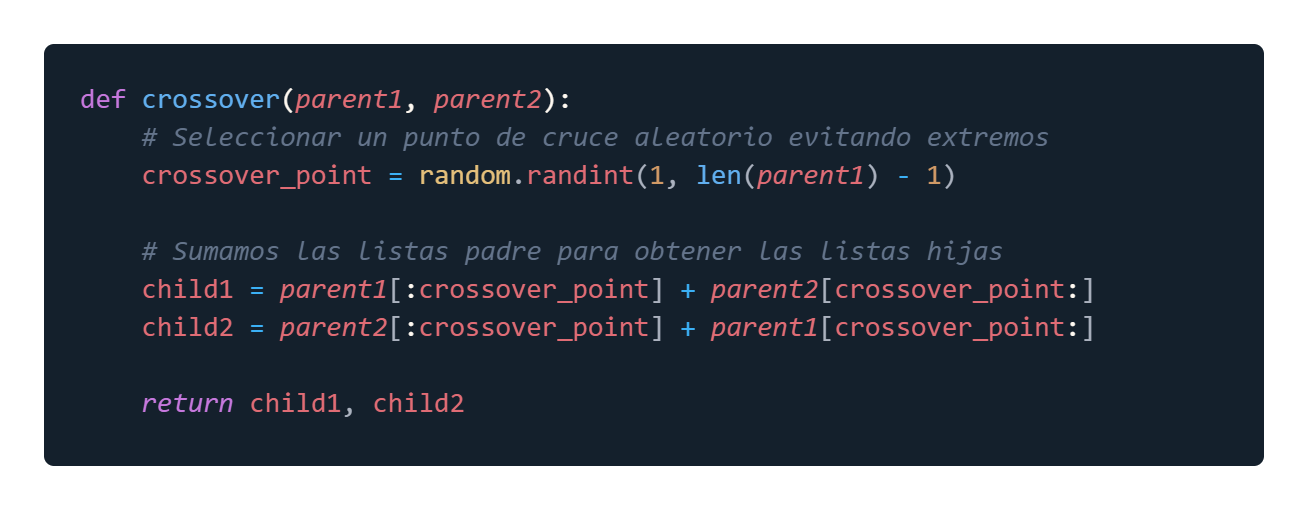
\includegraphics[width=0.5\textwidth]{funcionCruza.png}
        \caption{Función cruza}
    \end{figure}

    %Breve descripción del funcionamiento de la función
    La función cruza los individuos seleccionados para formar una nueva población.

    %Lista de parámetros
    \begin{itemize}
        \item padre 1: Es el primer individuo seleccionado para cruzarse.
        \item padre 2: Es el segundo individuo seleccionado para cruzarse.
    \end{itemize}

    %Descripción detallada del funcionamiento de la función
    La función esta diseñada para realizar una cruza entre dos individuos y generar dos hijos. 
    Esta empieza seleccionando un punto de cruza aleatorio, excluyendo el primero y el último índice de los individuos.
    Luego, crea dos hijos, el hijo 1 se crea utilizando la primera parte del padre 1 y la segunda parte del padre 2, 
    mientras que el hijo 2 se crea utilizando la primera parte del padre 2 y la segunda parte del padre 1.
    Finalmente, la función devuelve una lista con los dos hijos generados.

    \subsection*{Función de mutación}
    \begin{figure}[h]
        \centering
        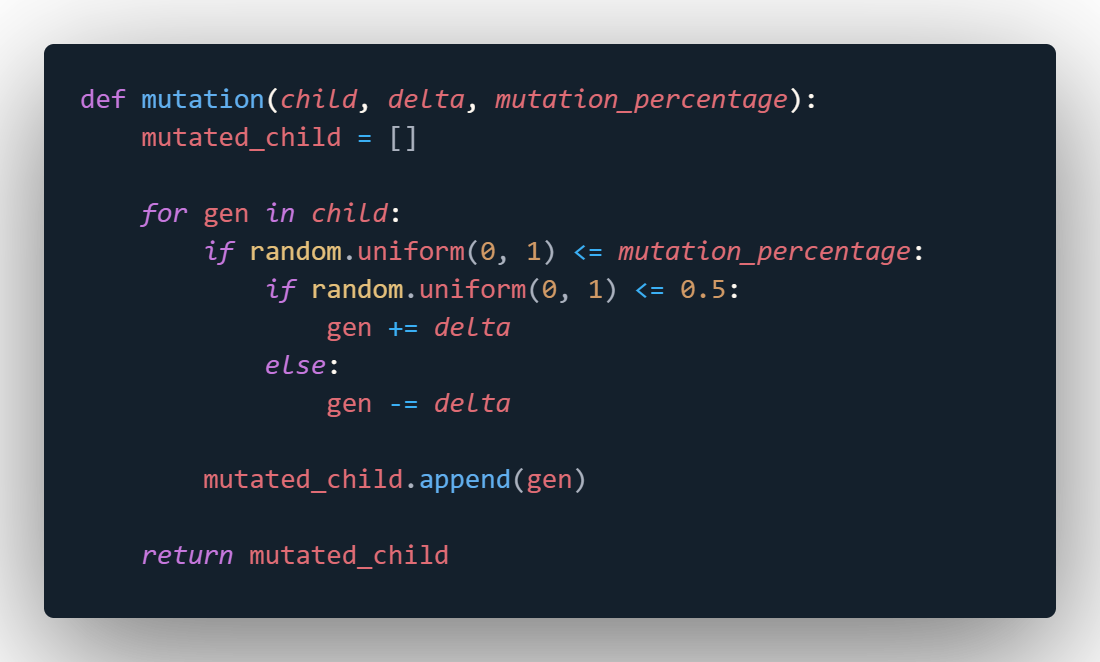
\includegraphics[width=0.5\textwidth]{funcionMutacion.png}
        \caption{Función mutación}
    \end{figure}

    %Breve descripción del funcionamiento de la función
    La función muta a los individuos de la población para mantener la diversidad en la población.

    %Lista de parámetros
    \begin{itemize}
        \item hijo: Es el individuo que se mutará.
        \item delta: Es el valor que se sumará o restará a cada variable del individuo.
        \item porcentaje de mutación: Es el porcentaje de individuos que se mutarán.
    \end{itemize}

    %Descripción detallada del funcionamiento de la función
    La función toma tres argumentos como entrada: el hijo, el delta y el porcentaje de mutación.
    El hijo es un individuo que se mutará, el delta es el valor que se sumará o restará a cada variable del individuo 
    y el porcentaje de mutación es el porcentaje de individuos que se mutarán.

    La función comienza creando una lista donde se guardarán los hijos mutados.
    Luego, se itera sobre cada gen del hijo y se decide si se muta o no.
    La mutación en si misma esta definida aleatoriamente por un valor entre 0 y 1, si este valor es menor al porcentaje de mutación.
    Aunque el gen este mutado o no este se guardara en la lista de hijos mutados.
    Finalmente, la función devuelve la lista de hijos mutados. 
    \newpage

    \subsection*{Función de creación de hijos}
    \begin{figure}[h]
        \centering
        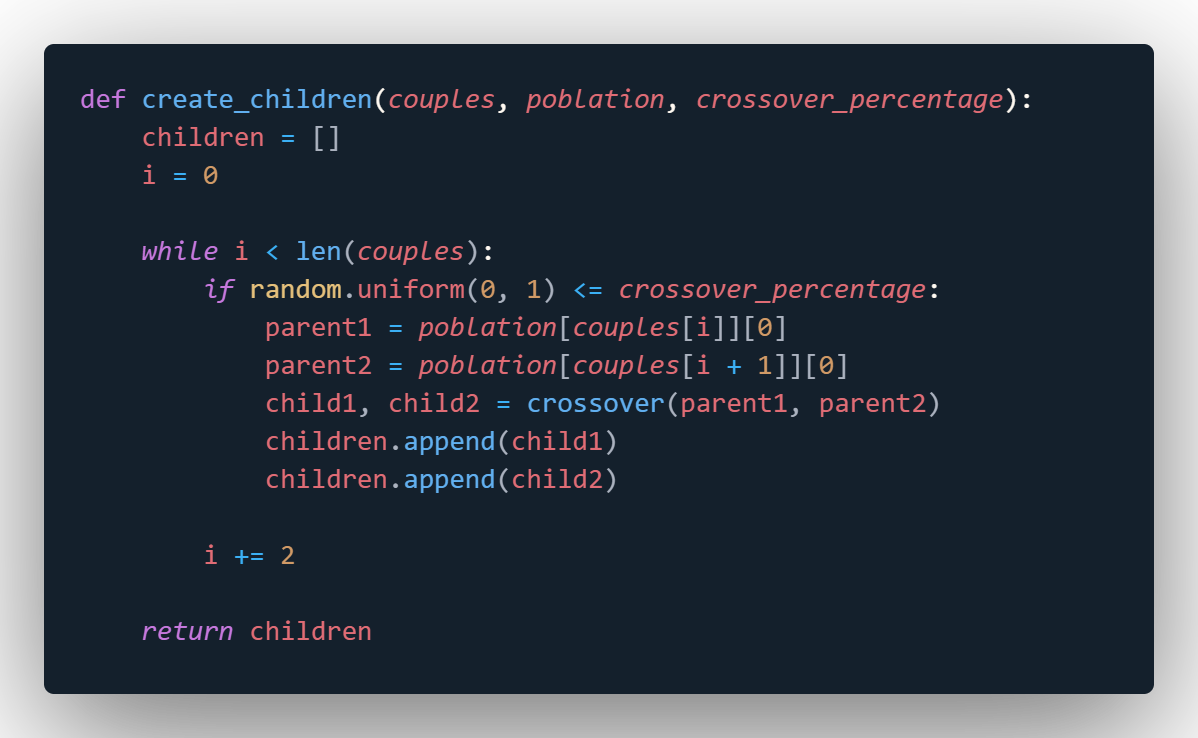
\includegraphics[width=0.5\textwidth]{funcionSeleccion.png}
        \caption{Función hijos}
    \end{figure}

    %Breve descripción del funcionamiento de la función
    La función crea hijos a partir de los individuos seleccionados la población y el porcentaje de cruza.

    %Lista de parámetros
    \begin{itemize}
        \item población: Es la lista de individuos que se cruzarán.
        \item parejas: Es la lista de índices de los individuos seleccionados.
        \item porcentaje de cruza: Es el porcentaje de individuos que se cruzarán.
    \end{itemize}

    %Descripción detallada del funcionamiento de la función
    La función esta diseñada de tal forma que crea una nueva generación de individuos 
    a partir de la población actual.
    Esta toma tres argumentos como entrada: la población, las parejas y el porcentaje de cruza.

    La función inicia creando una lista de hijos vacía, donde se almacenarán los hijos generados.
    Después, la función entra en un ciclo while que se ejecuta hasta que el iterador sea menor que el número de parejas.
    Dentro del ciclo genera números aleatorios entre 0 y 1, si el número es menor al porcentaje de cruza, si el numero es menor o igual
    al porcentaje de cruza, se selecciona a los individuos de la población que se cruzarán y se cruzan.

    Los padres seleccionados desde la población usando los indices proporcionados por la función de selección de parejas se cruzarán y se generaran dos hijos.
    Los nuevos individuos serás indexados a la lista de hijos, se incrementará el iterador por dos y se repetirá el proceso hasta que se hayan terminado los indices de selección.

    Finalmente, después de que se hayan procesado toda la lista de parejas, la función devuelve la lista de hijos generados.

    \subsection*{Función del algoritmo genético}

    %Agrega la imagen de la función
    \begin{figure}[h]
        \centering
        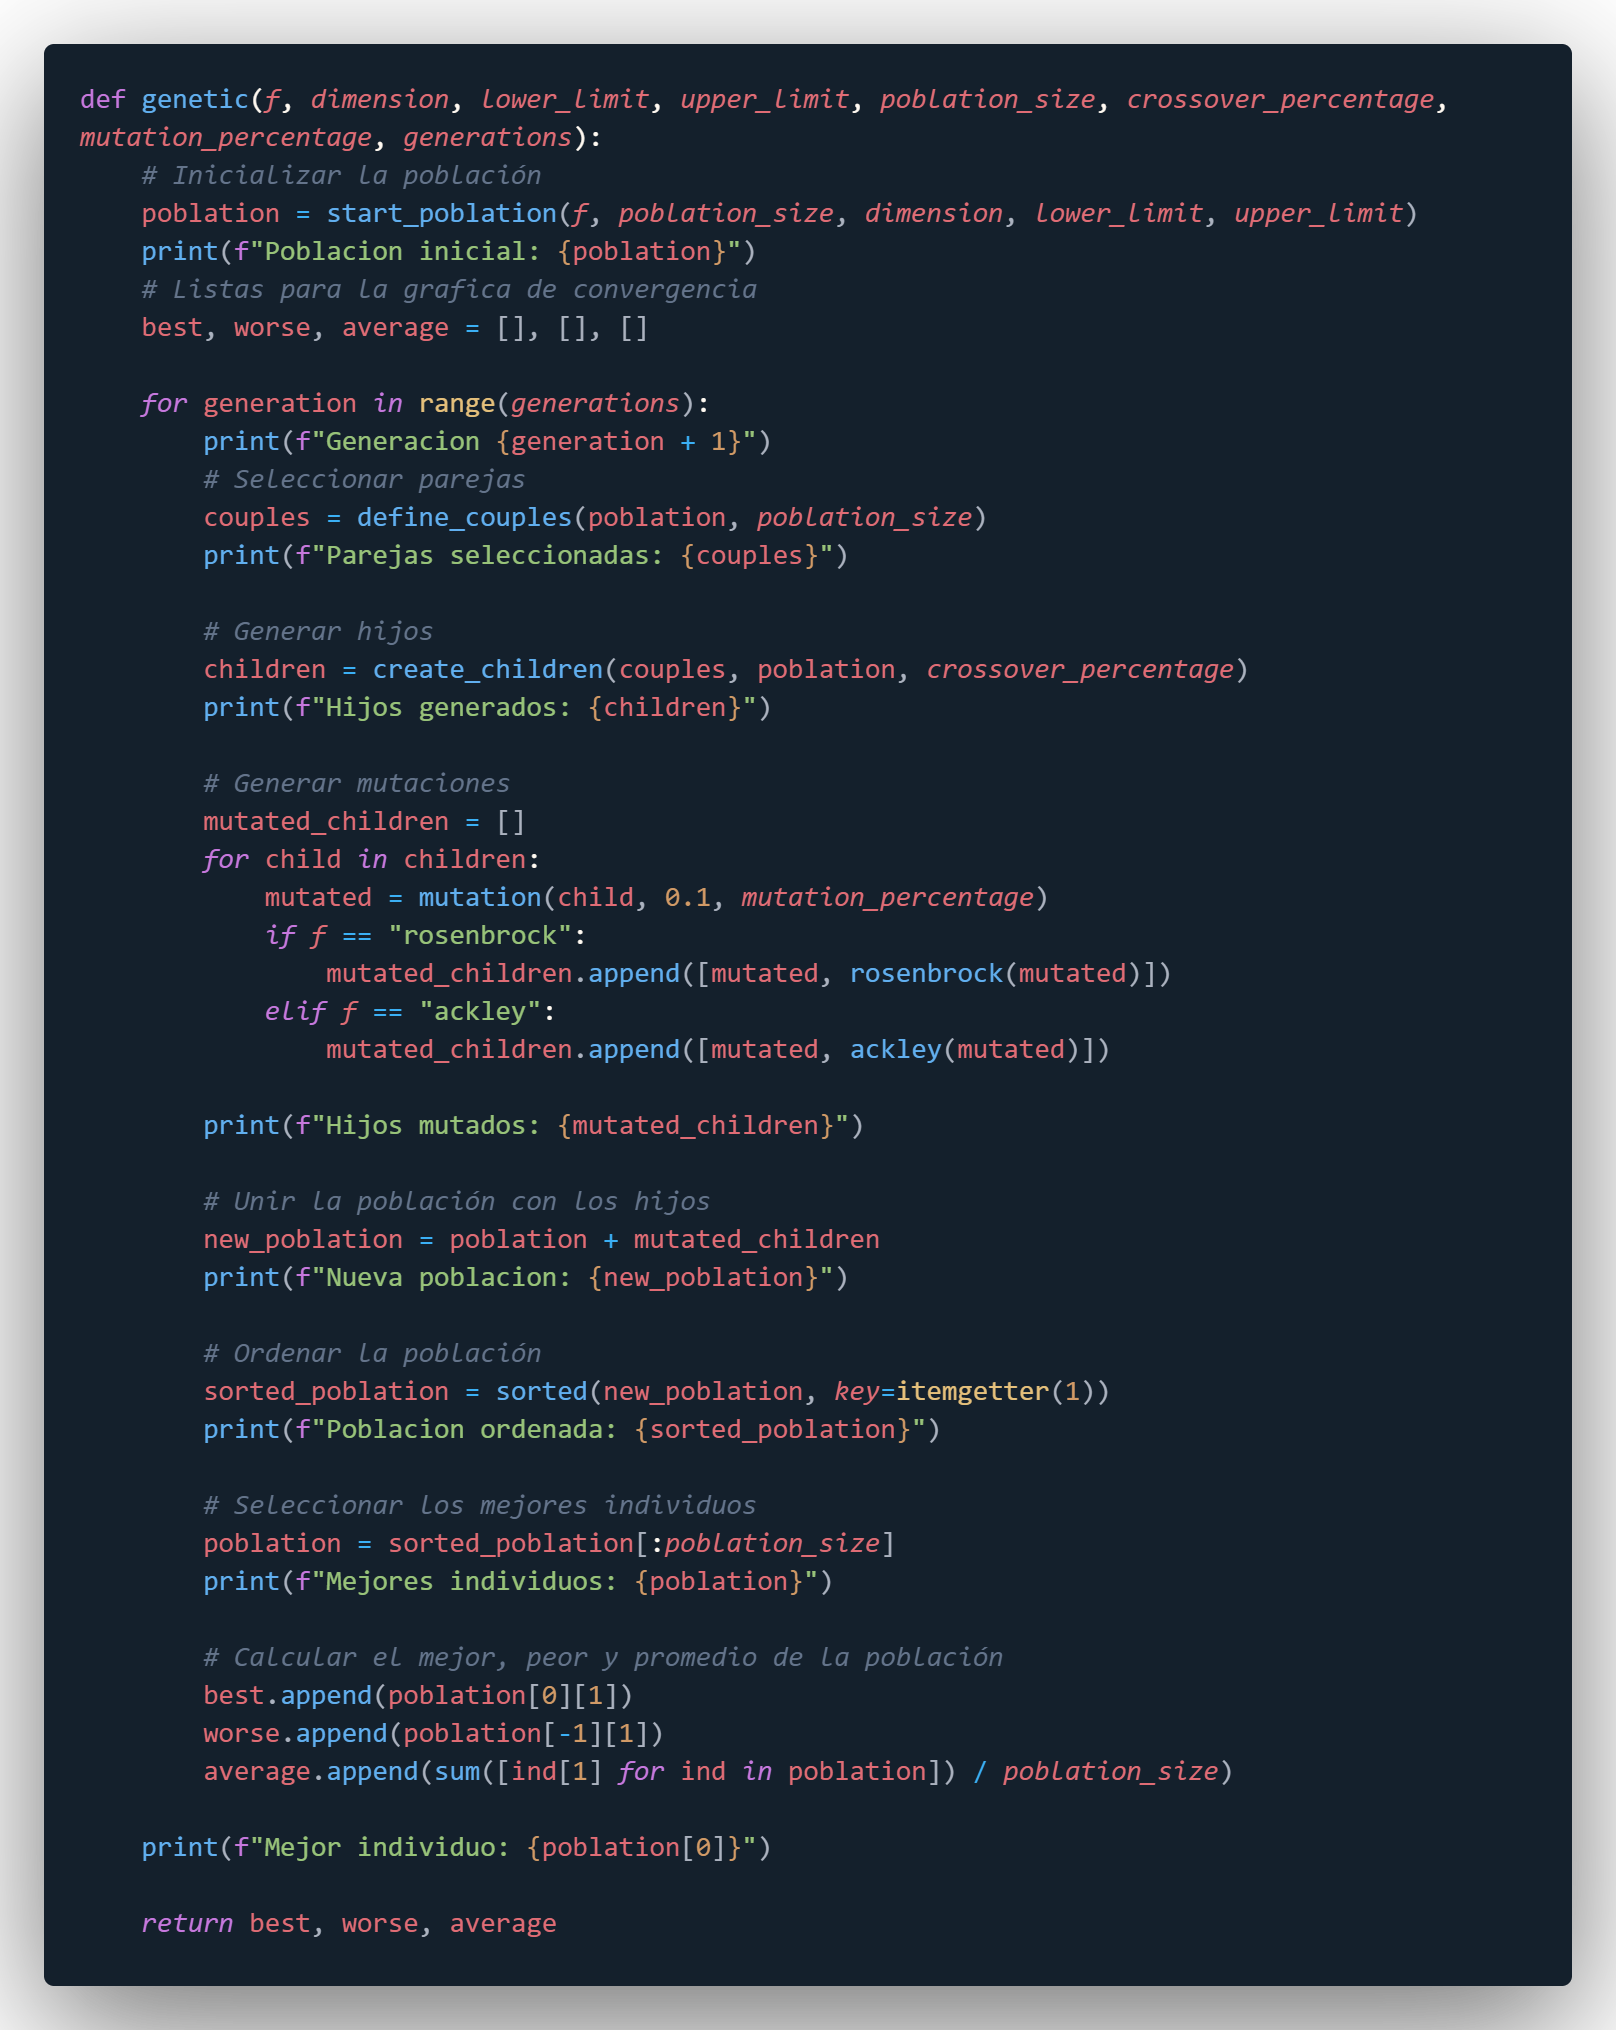
\includegraphics[width=0.5\textwidth]{funcionGenetico.png}
        \caption{Función algoritmo genético}
    \end{figure}

    %Breve descripción del funcionamiento de la función
    La función principal del algoritmo genético, esta función se encarga de ejecutar el algoritmo genético.

    %Descripción de los parámetros de la función
    \begin{itemize}
        \item f: Es una cadena que especifica la función de aptitud que se utilizará, ya sea Rosenbrock o Ackley.
        \item tamaño de la población: Es el número de individuos que se generarán.
        \item dimensión: Es el número de variables que tendrá cada individuo.
        \item limite inferior: Es el valor mínimo que pueden tomar las variables de cada individuo.
        \item limite superior: Es el valor máximo que pueden tomar las variables de cada individuo.
        \item porcentaje de cruza: Es el porcentaje de individuos que se cruzarán.
        \item porcentaje de mutación: Es el porcentaje de individuos que se mutarán.
        \item generaciones: Es el número de generaciones que se ejecutarán.
    \end{itemize}

    %Descripción detallada del funcionamiento de la función
    La función comienza inicializando una población de individuos utilizando la función de inicialización de población. Cada individuo de la
    población se evalúa utilizando la función de aptitud especificada. La función de aptitud devuelve un valor que representa la aptitud del individuo.

    Posteriormente, para cada generación, evalúa cada generación con los siguientes pasos:
    %crea una lista ordenada
    \begin{itemize}
        \item Selecciona las parejas de individuos que se cruzarán utilizando la función de selección de acuerdo a su fitness, mediante el algoritmo de la ruleta.
        \item Crea una nueva generación de individuos a partir de la población actual utilizando la función de creación de hijos.
        \item Muta a los individuos de la nueva generación utilizando la función de mutación.
        \item Evalúa la nueva generación de individuos utilizando la función de aptitud.
        \item Ordena los individuos según su aptitud.
        \item Selecciona los mejores individuos para la siguiente generación.
        \item Guarda el mejor, el peor y la aptitud media de la generación para su graficación posterior.
    \end{itemize}

    Finalmente, terminando todas las generaciones, la función muestra los resultados del mejor individuo, el peor individuo y la aptitud media de cada generación.

    \newpage

    \section*{Resultados}
    \subsection*{Función de Rosenbrock Real}
    \begin{figure}[h]
        \centering
        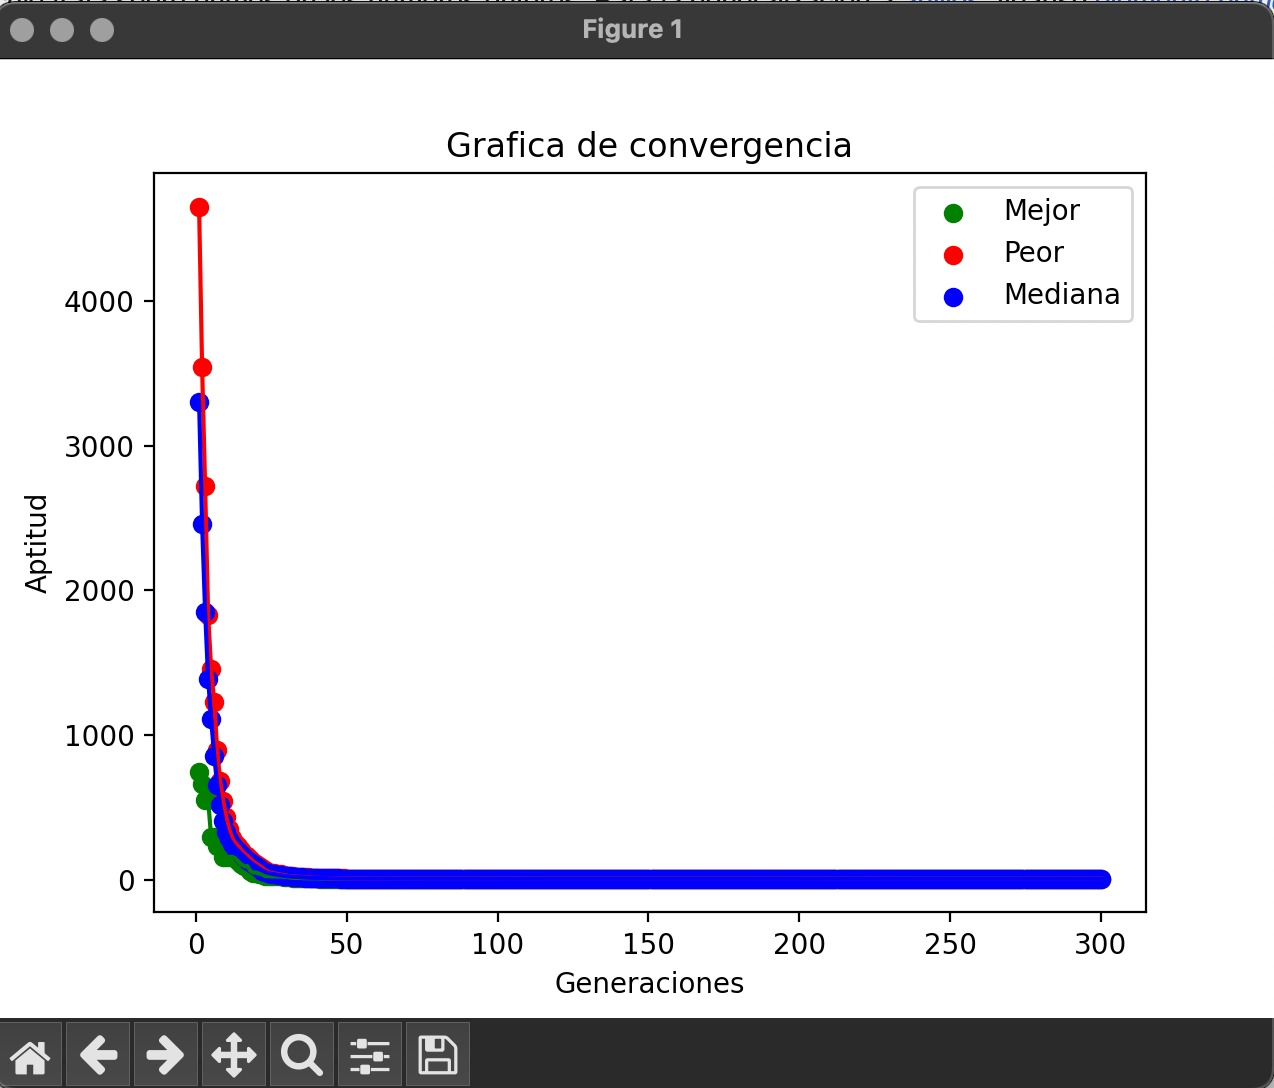
\includegraphics[width=0.5\textwidth]{rosenbrock_7_re.jpeg}
        \caption{Rosenbrock, semilla= 7, Real}
    \end{figure}

    \begin{figure}[p]
        \centering
        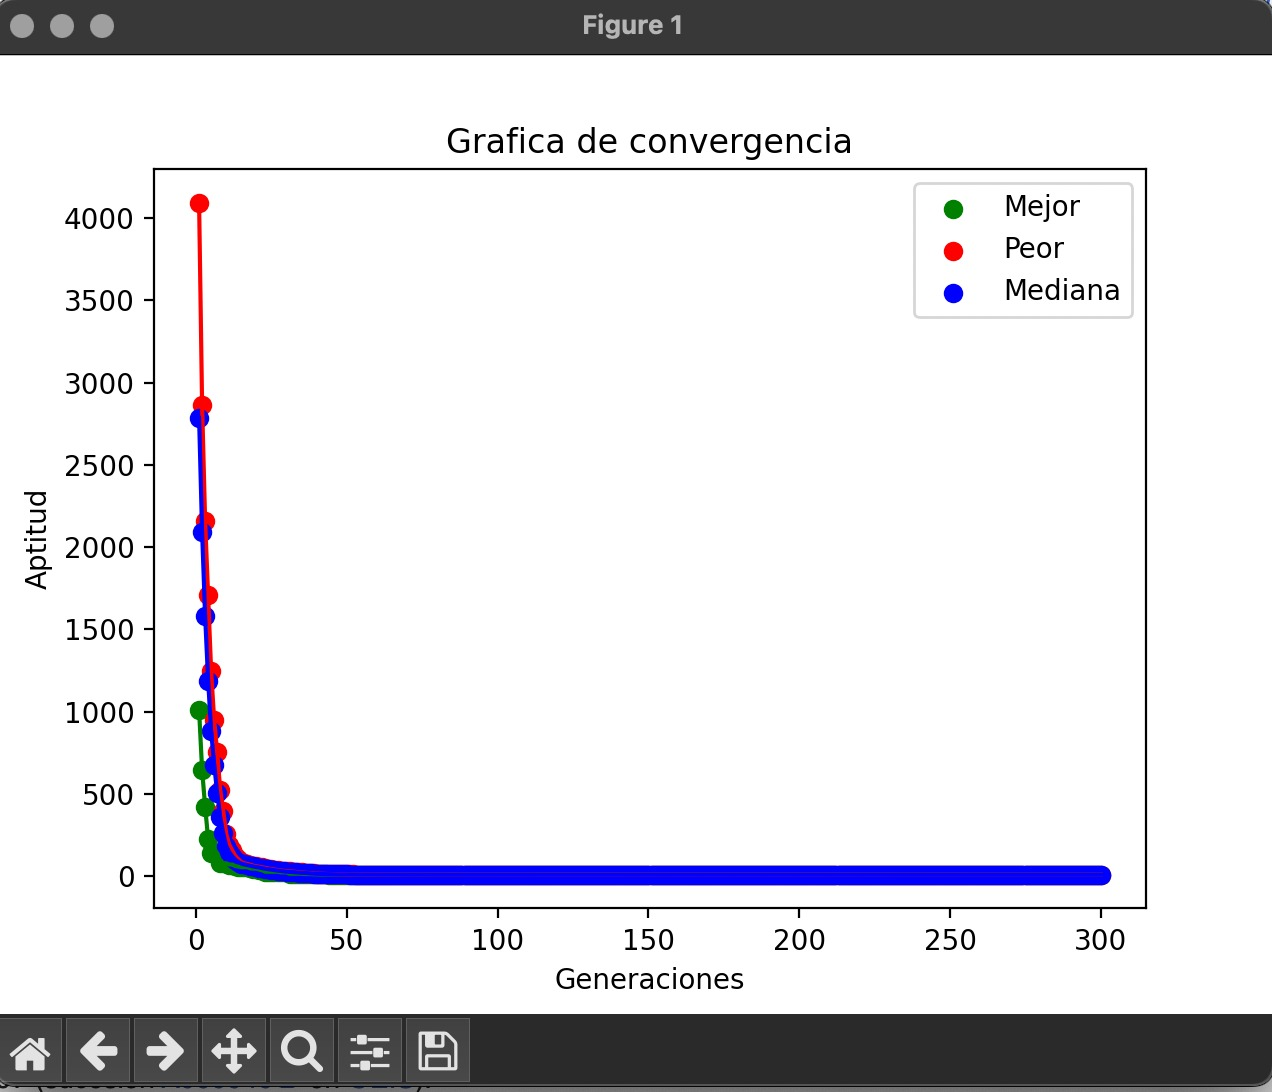
\includegraphics[width=0.5\textwidth]{rosenbrock_11_re.jpeg}
        \caption{Rosenbrock, semilla= 11, Real}
    \end{figure}

    \begin{figure}[p]
        \centering
        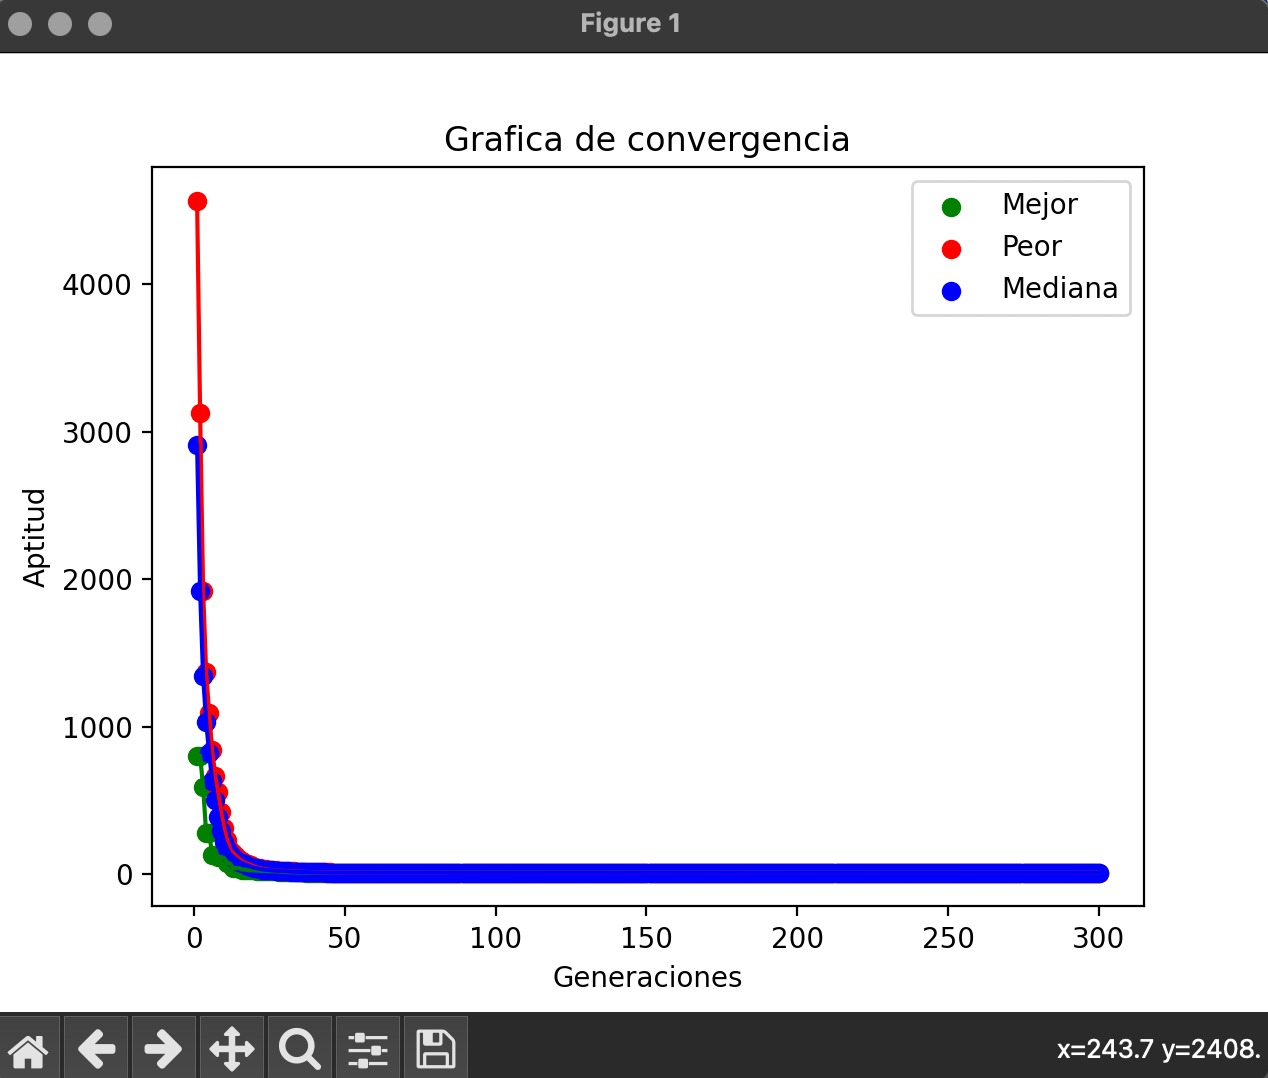
\includegraphics[width=0.5\textwidth]{rosenbrock_61_re.jpeg}
        \caption{Rosenbrock, semilla= 61, Real}
    \end{figure}

    \subsection*{Función de Rosenbrock Binaria} 

    \begin{figure}[h]
        \centering
        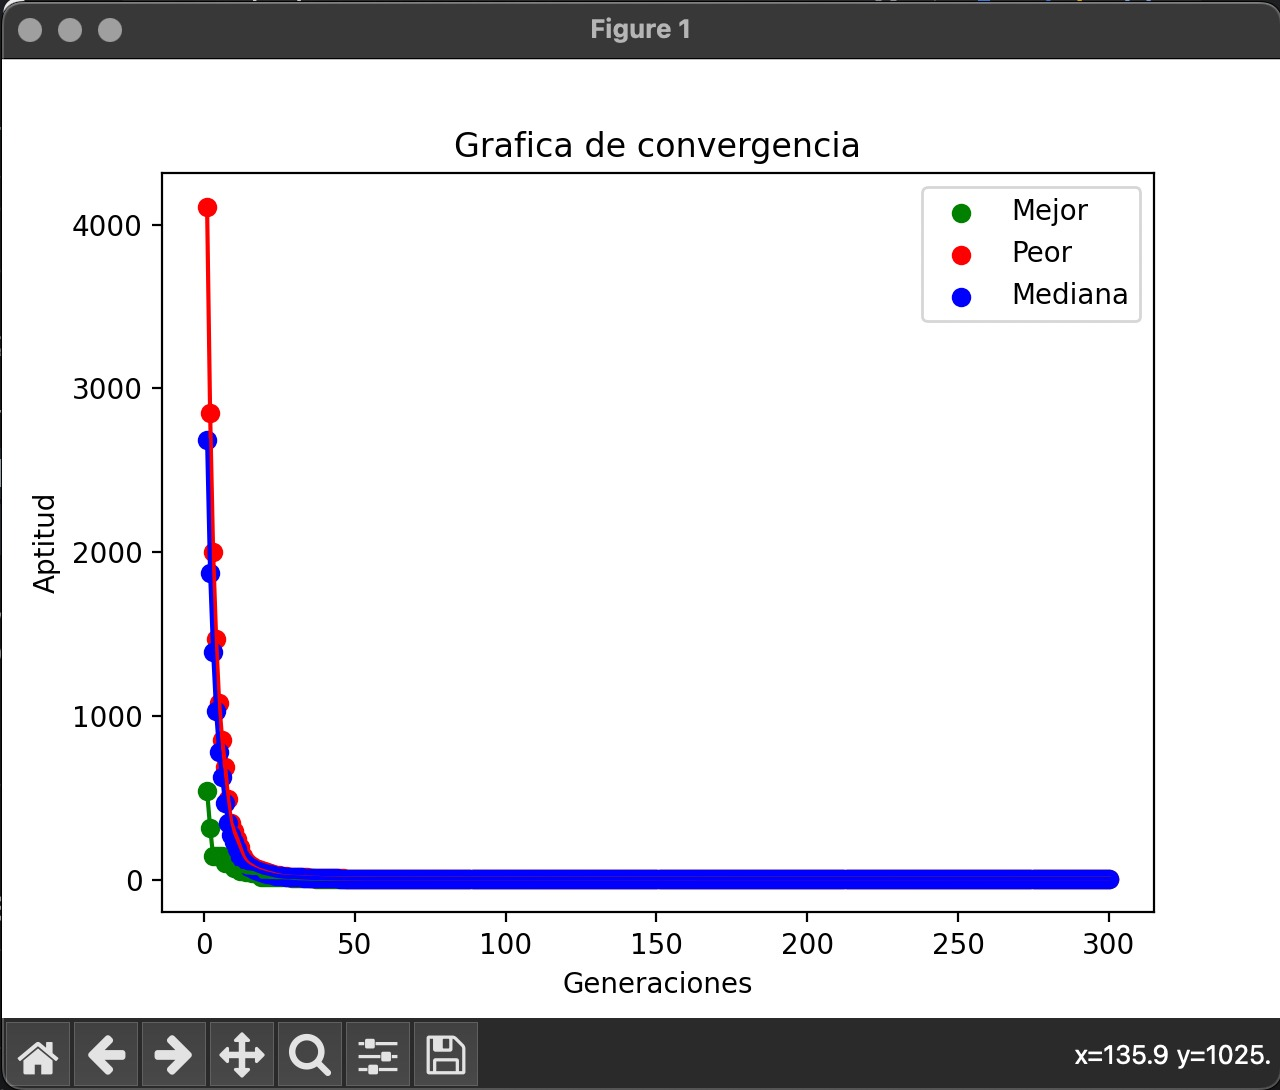
\includegraphics[width=0.5\textwidth]{rosenbrock_59_bin.jpeg}
        \caption{Rosenbrock, semilla= 59, Binaria}
    \end{figure}

    \begin{figure}[p]
        \centering
        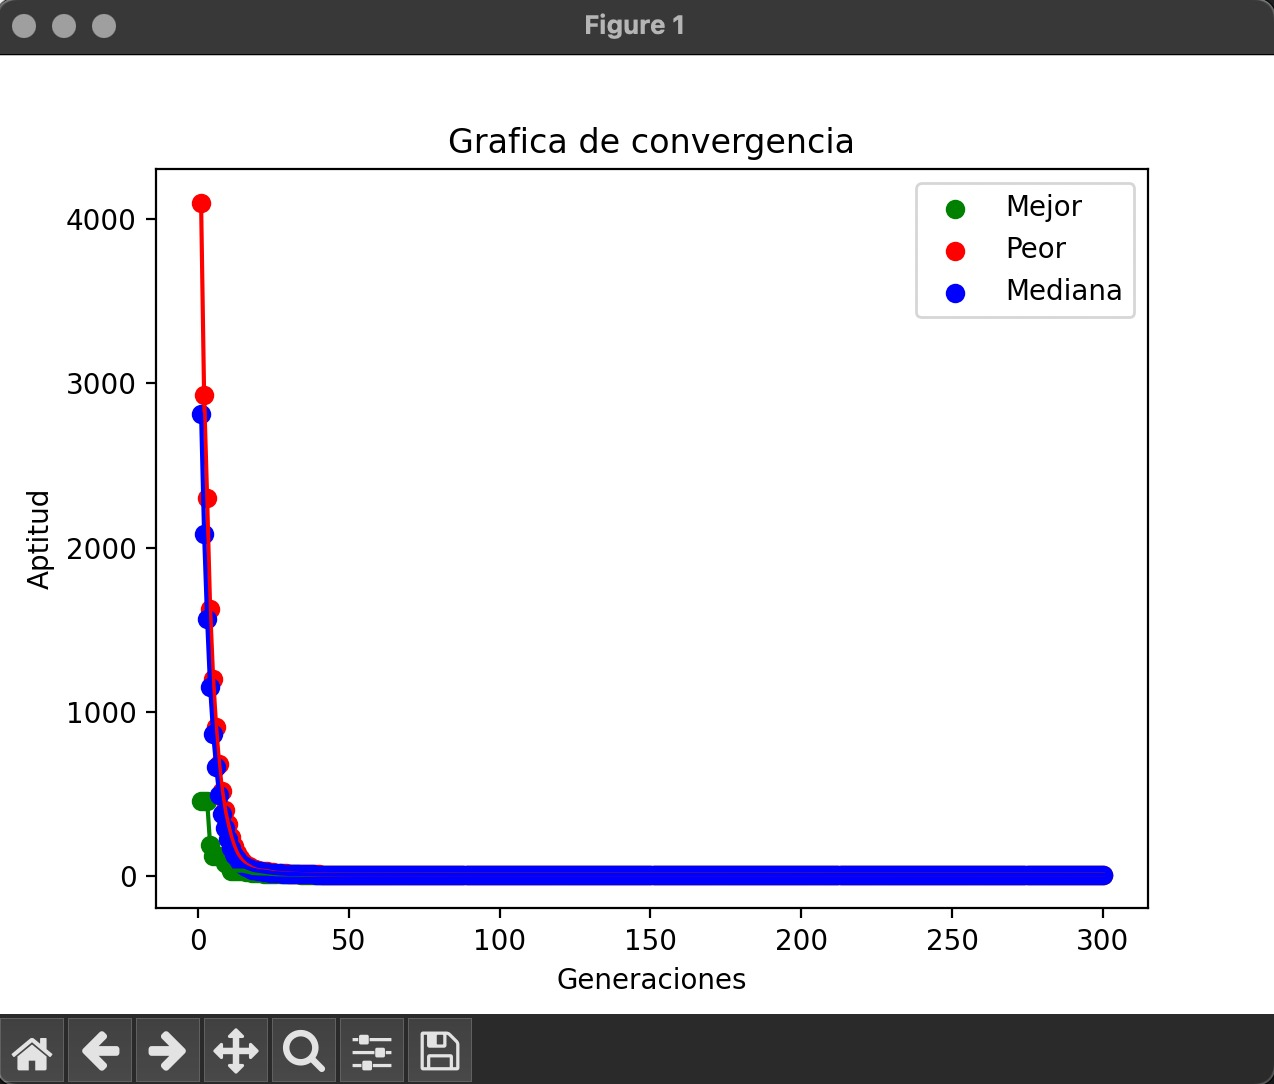
\includegraphics[width=0.5\textwidth]{rosenbrock_79_bin.jpeg}
        \caption{Rosenbrock, semilla= 79, Binaria}
    \end{figure}

    \begin{figure}[p]
        \centering
        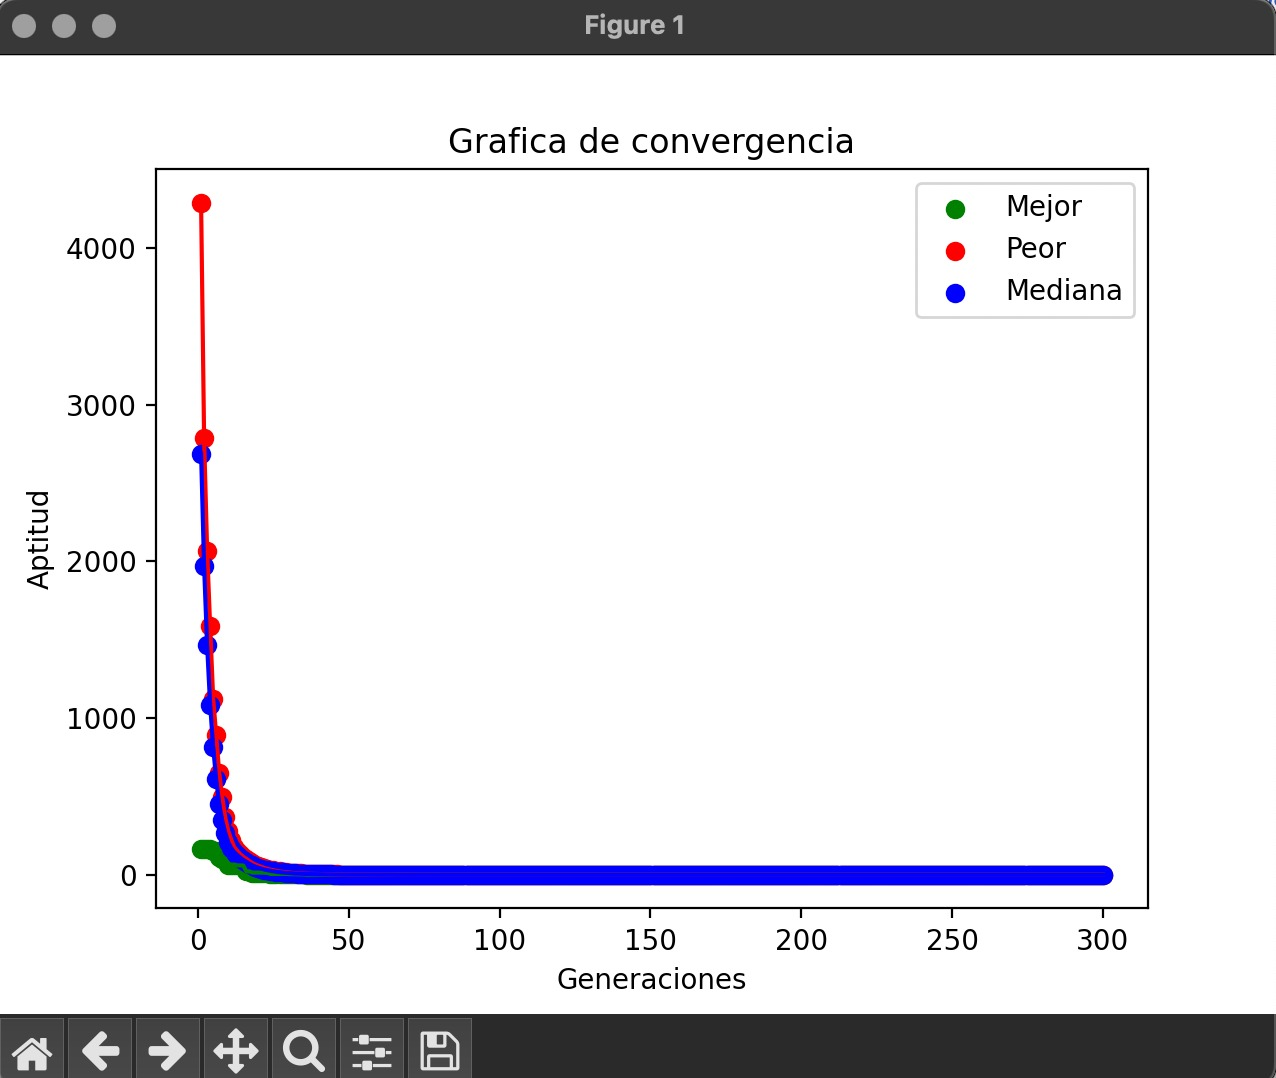
\includegraphics[width=0.5\textwidth]{rosenbrock_97_bin.jpeg}
        \caption{Rosenbrock, semilla= 97, Binaria}
    \end{figure}

    \subsection*{Función de Ackley Real}
    
    \begin{figure}[h]
        \centering
        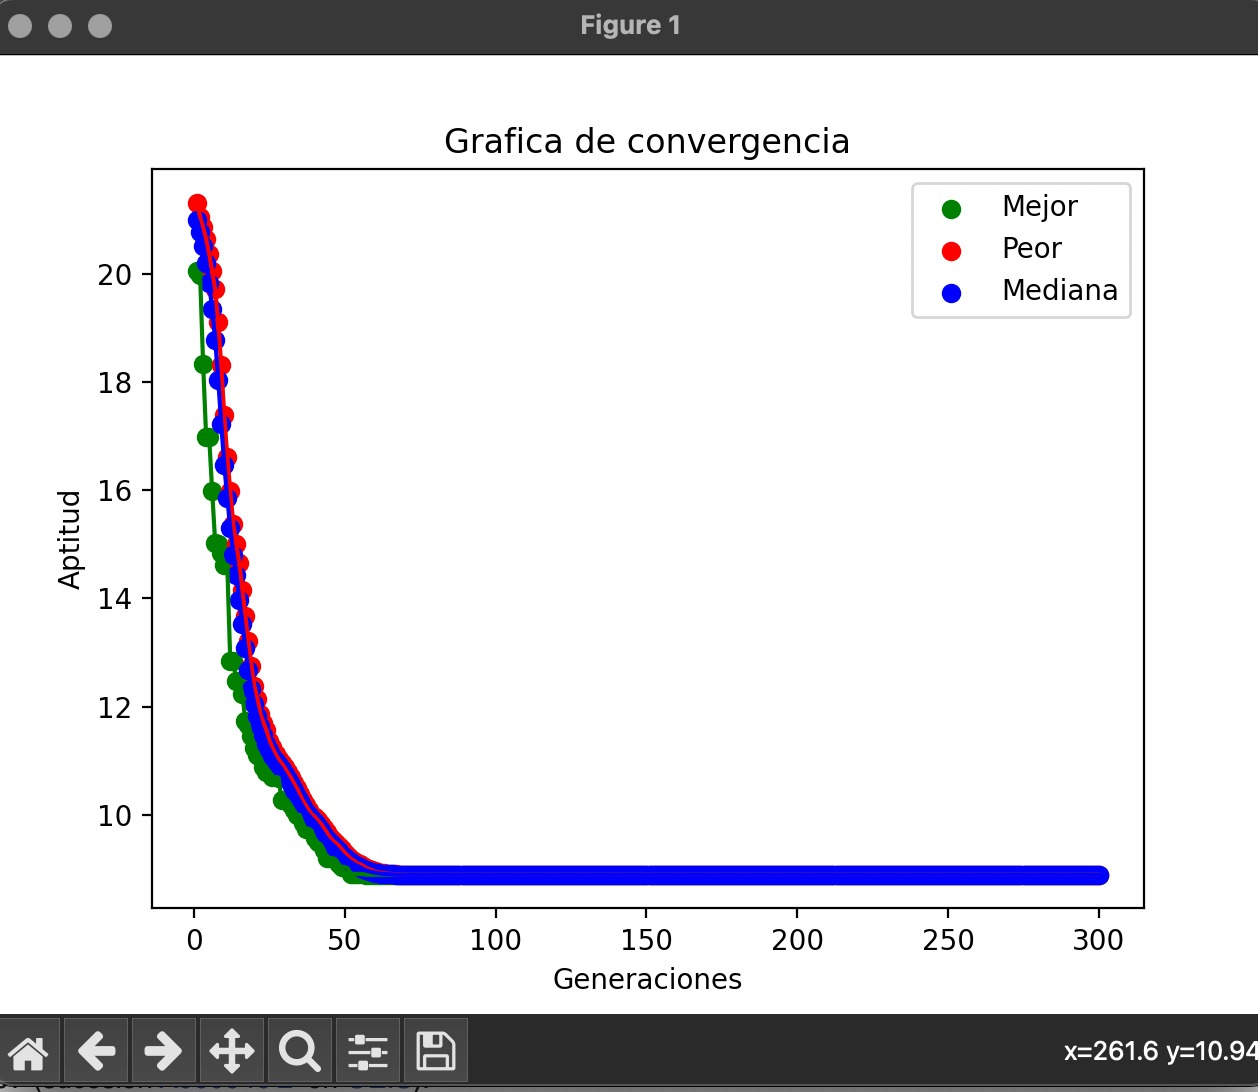
\includegraphics[width=0.5\textwidth]{ackley_7_re.jpeg}
        \caption{Ackley, semilla= 7, Real}
    \end{figure}
    \begin{figure}[p]
        \centering
        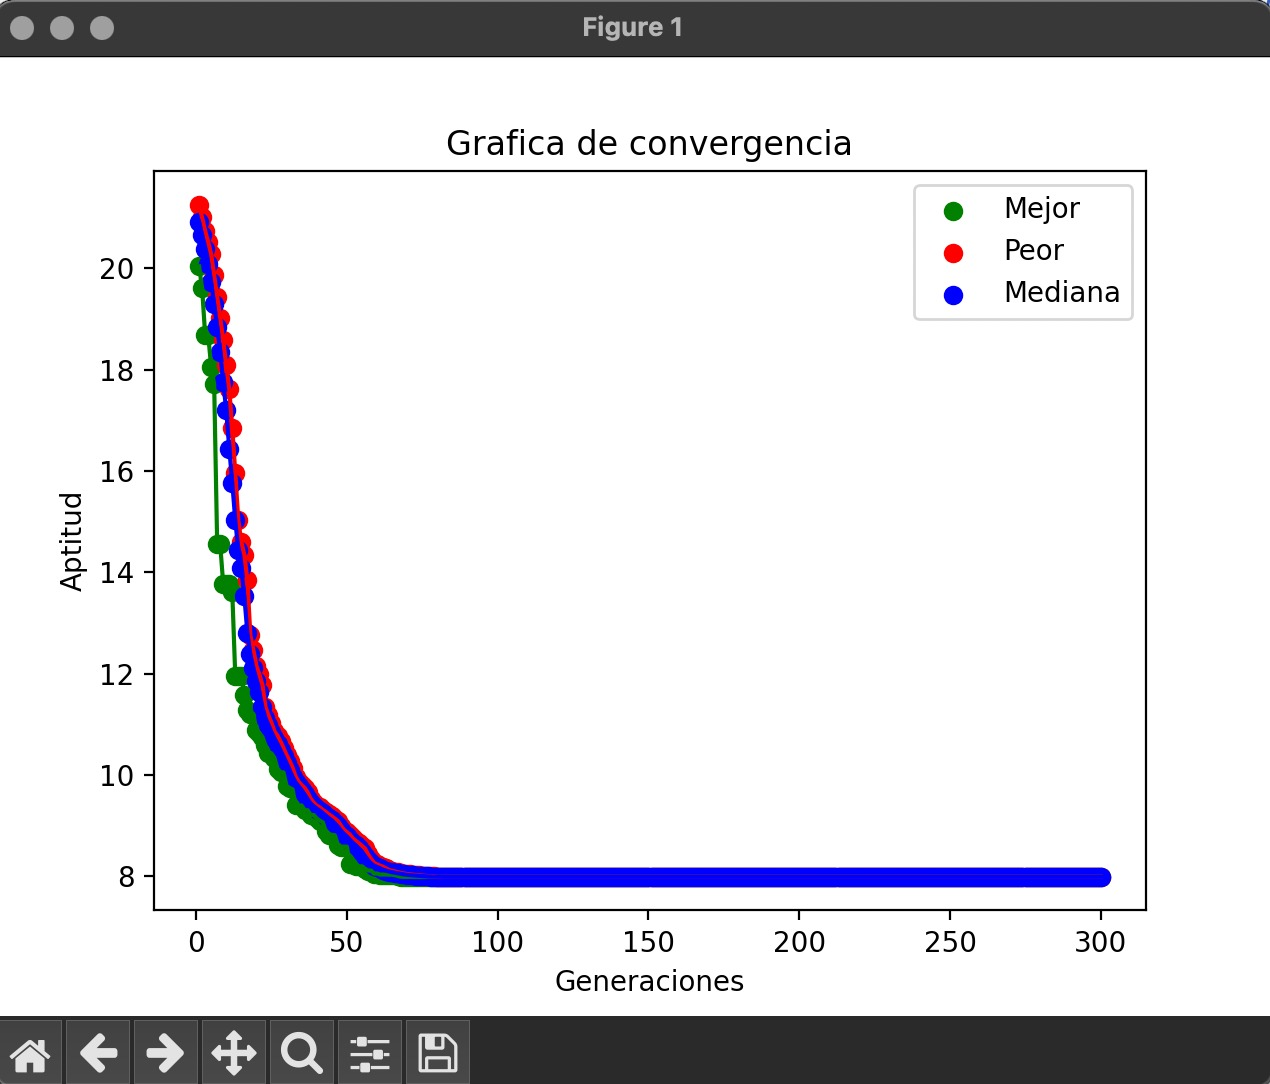
\includegraphics[width=0.5\textwidth]{ackley_97_re.jpeg}
        \caption{Ackley, semilla= 97, Real}
    \end{figure}

    \begin{figure}[p]
        \centering
        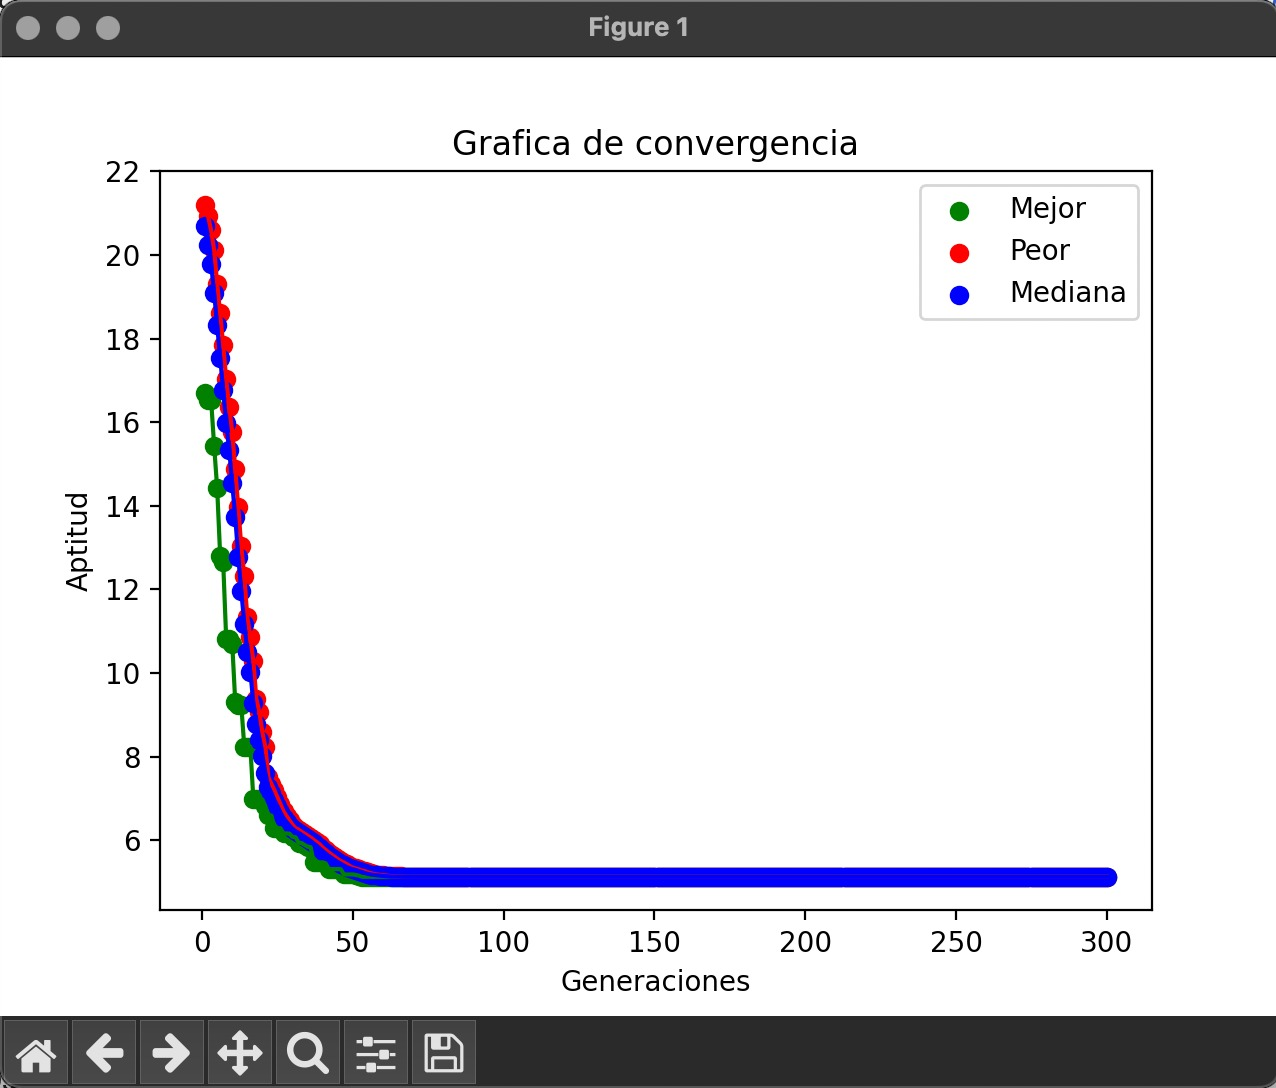
\includegraphics[width=0.5\textwidth]{ackley_113_re.jpeg}
        \caption{Ackley, semilla= 113, Real}
    \end{figure}
    
    \subsection*{Función de Ackley Binaria}
    
    \begin{figure}[h]
        \centering
        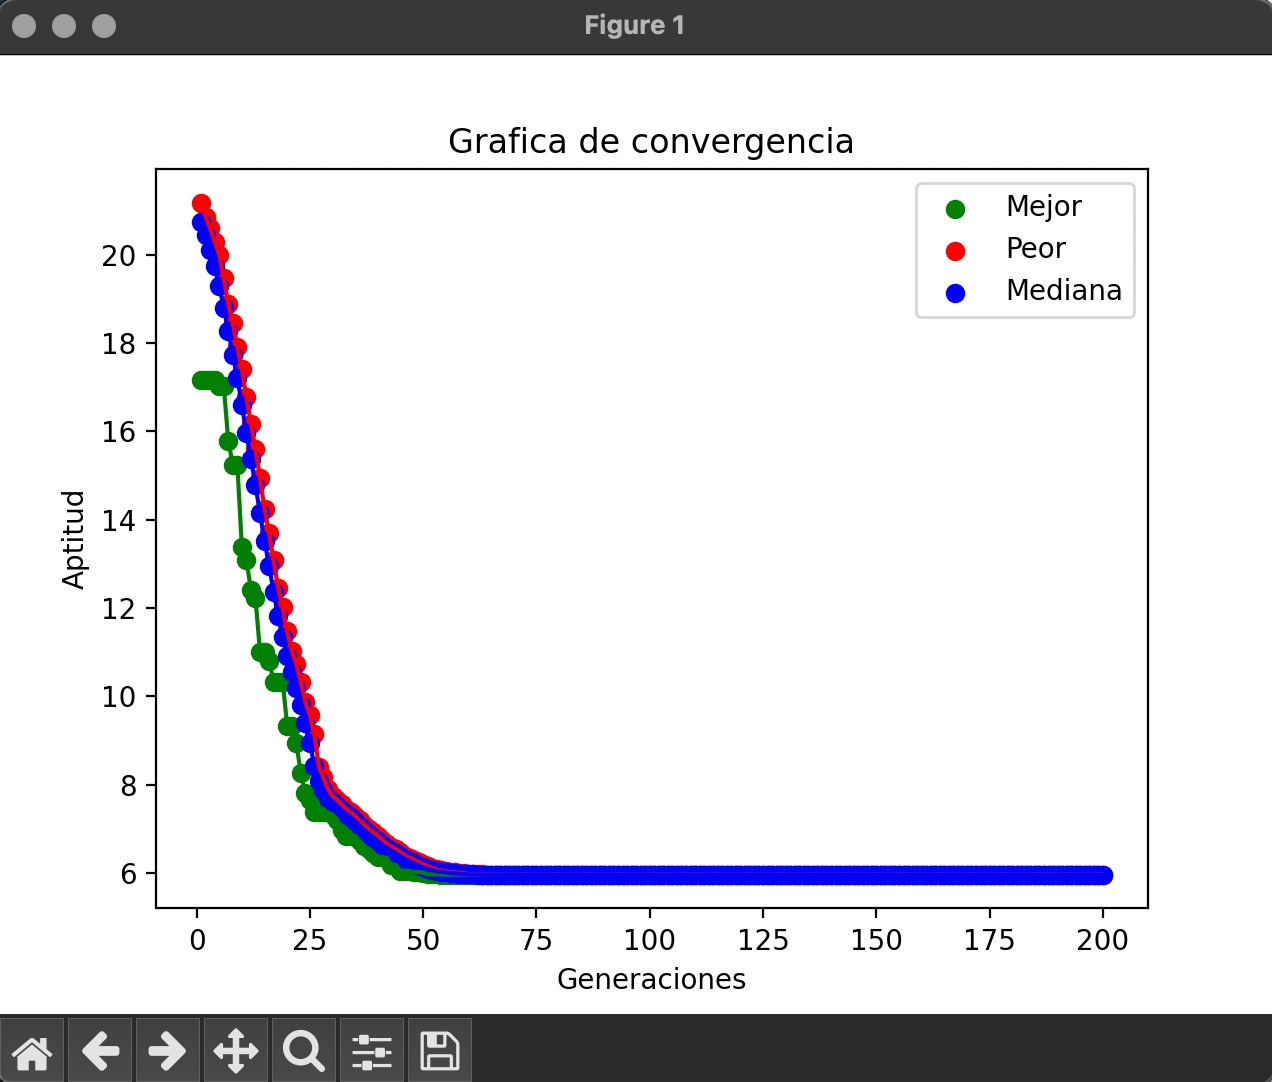
\includegraphics[width=0.5\textwidth]{ackley_13_bin.jpeg}
        \caption{Ackley, semilla= 13, Binaria}
    \end{figure}
    \begin{figure}[p]
        \centering
        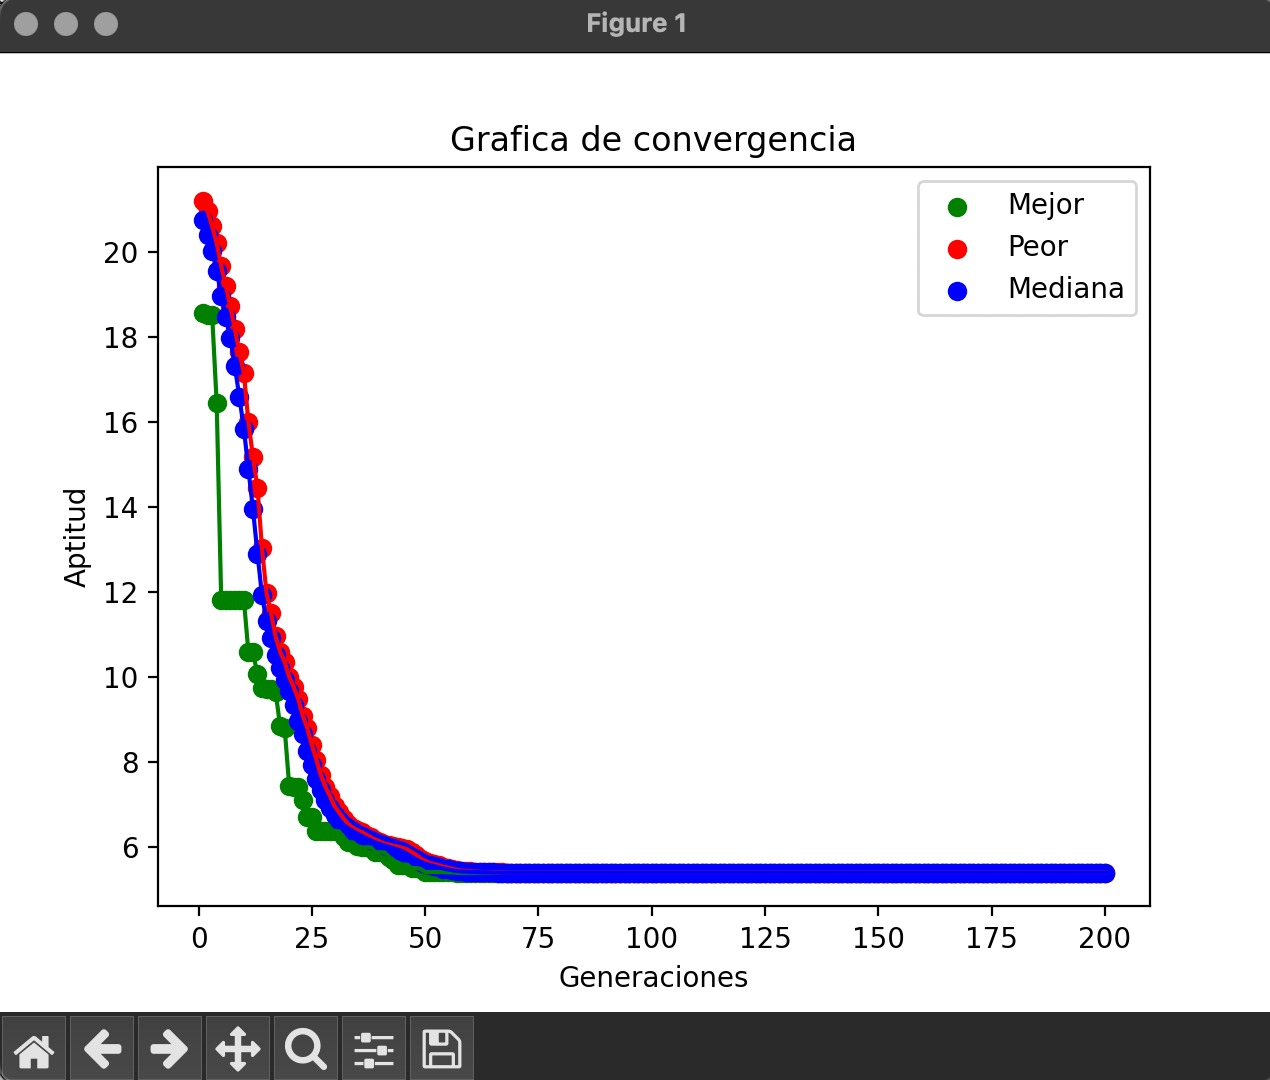
\includegraphics[width=0.5\textwidth]{ackley_83_bin.jpeg}
        \caption{Ackley, semilla= 83, Binaria}
    \end{figure}
    \begin{figure}[p]
        \centering
        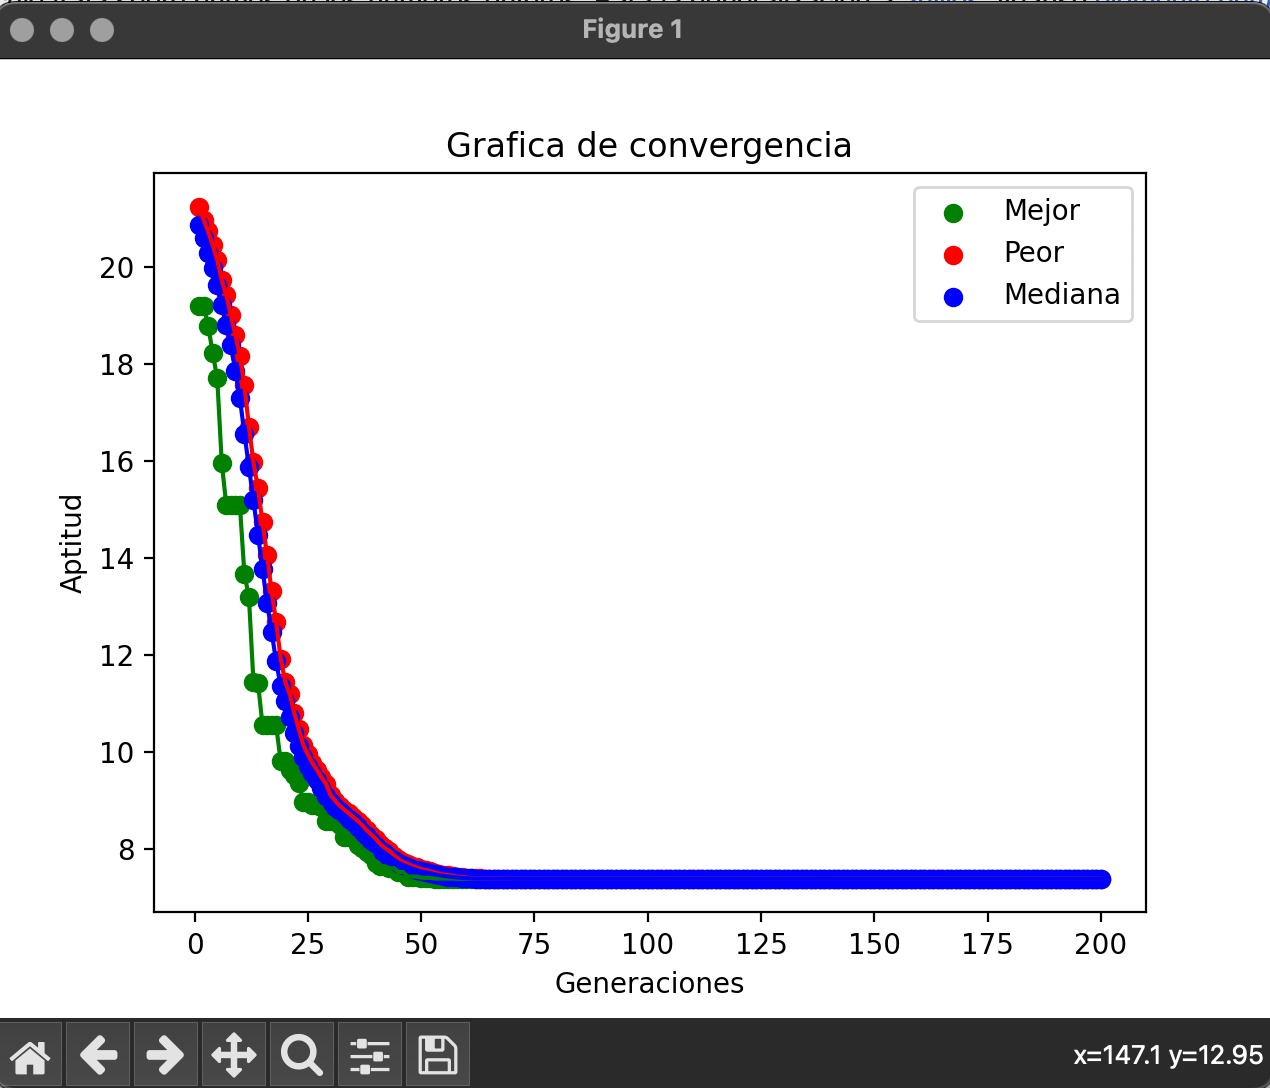
\includegraphics[width=0.5\textwidth]{ackley_101_bin.jpeg}
        \caption{Ackley, semilla= 101, Binaria}
    \end{figure}

\end{document}